\documentclass[aspectratio=169,10pt]{beamer}
\usetheme{Madrid}
\usecolortheme{default}

\usepackage{amsmath}
\usepackage{amssymb}
\usepackage{booktabs}
\usepackage{graphicx}
\usepackage{subcaption} % for subfigure
\usepackage{tikz}
\usepackage{tcolorbox}
\usetikzlibrary{arrows,positioning,shapes,backgrounds,fit, calc}
\usepackage{pgfplots}
\pgfplotsset{compat=1.18}

% Custom colors
\definecolor{darkblue}{RGB}{0,51,102}
\definecolor{lightblue}{RGB}{51,153,255}
\definecolor{darkgreen}{RGB}{0,102,51}
\definecolor{orange}{RGB}{255,128,0}
\definecolor{darkred}{RGB}{153,0,0}

\setbeamercolor{structure}{fg=darkblue}
\setbeamercolor{frametitle}{bg=darkblue,fg=white}

\title{LOM: A Large Optimization Model for Near-Real Time Large-Scale Power System Flexibility Scenario Exploration}
\author{Théotime Coudray \& Stéphane Goutte}
\institute{UVSQ - PowDev}
\date{\today}

\begin{document}

% Title slide
\begin{frame}
\titlepage
\end{frame}


\section{Problem Motivation}

\begin{frame}{The Unit Commitment Challenge}
\begin{columns}
\column{0.5\textwidth}
\textbf{What is Unit Commitment?}
\begin{itemize}
    \item Optimize power system operations over 24h, at 15 min time resolution
    \item Decide which generators to turn on/off
    \item Schedule generation to meet demand
    \item Minimize total system cost
\end{itemize}

\vspace{1em}
\textbf{Why is it Hard?}
\begin{itemize}
    \item Mixed-Integer Linear Program (MILP)
    \item NP-hard combinatorial problem
    \item Large-scale: 100+ zones, 96 timesteps
    \item Hours to solve with commercial solvers
\end{itemize}

\column{0.5\textwidth}
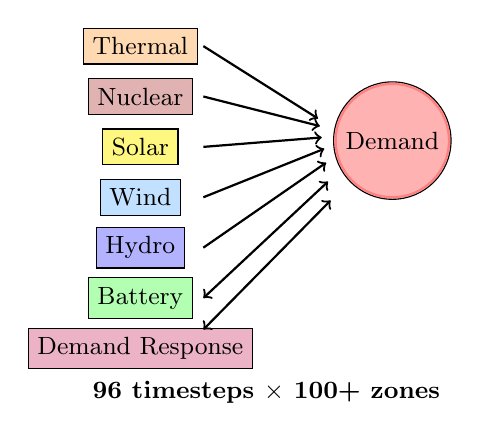
\begin{tikzpicture}[scale=0.8]
    % Generators
    \node[draw,rectangle,fill=orange!30] at (0,3) {\small Thermal};
    \node[draw,rectangle,fill=darkred!30] at (0,2.2) {\small Nuclear};
    \node[draw,rectangle,fill=yellow!50] at (0,1.4) {\small Solar};
    \node[draw,rectangle,fill=lightblue!30] at (0,0.6) {\small Wind};
    \node[draw,rectangle,fill=blue!30] at (0,-0.2) {\small Hydro};
    \node[draw,rectangle,fill=green!30] at (0,-1.0) {\small Battery};
    \node[draw,rectangle,fill=purple!30] at (0,-1.8) {\small Demand Response};
    
    % Demand with surrounding circle
    \node[draw,circle,fill=red!30,minimum size=0.8cm] (demand_inner) at (4,1.5) {\small Demand};
    \draw[thick,red!50] (4,1.5) circle (0.9cm);
    
    % Connections - arrows point to outer circle
    \draw[->,thick] (1,3) -- (2.82,1.85);
    \draw[->,thick] (1,2.2) -- (2.85,1.73);
    \draw[->,thick] (1,1.4) -- (2.88,1.55);
    \draw[->,thick] (1,0.6) -- (2.92,1.37);
    \draw[->,thick] (1,-0.2) -- (2.95,1.15);
    \draw[<->,thick] (1,-1.0) -- (2.98,0.85);
    \draw[<->,thick] (1,-1.5) -- (3.02,0.55);
    
    \node at (2,-2.5) {\small \textbf{96 timesteps $\times$ 100+ zones}};
\end{tikzpicture}
\end{columns}
\end{frame}

\begin{frame}{Asset-Level Complexity}
\begin{center}
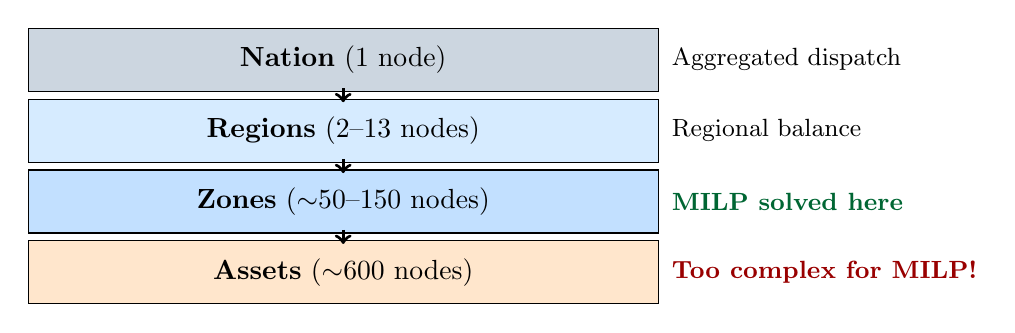
\begin{tikzpicture}[scale=0.9]
    % Hierarchy
    \node[draw,rectangle,fill=darkblue!20,minimum width=8cm,minimum height=0.8cm] at (0,3) {\textbf{Nation} (1 node)};
    \node[draw,rectangle,fill=lightblue!20,minimum width=8cm,minimum height=0.8cm] at (0,2) {\textbf{Regions} (2--13 nodes)};
    \node[draw,rectangle,fill=lightblue!30,minimum width=8cm,minimum height=0.8cm] at (0,1) {\textbf{Zones} ($\sim$50--150 nodes)};
    \node[draw,rectangle,fill=orange!20,minimum width=8cm,minimum height=0.8cm] at (0,0) {\textbf{Assets} ($\sim$600 nodes)};
    
    % Arrows
    \draw[->,very thick] (0,2.6) -- (0,2.4);
    \draw[->,very thick] (0,1.6) -- (0,1.4);
    \draw[->,very thick] (0,0.6) -- (0,0.4);
    
    % Annotations
    \node[align=left,anchor=west] at (4.5,3) {\small Aggregated dispatch};
    \node[align=left,anchor=west] at (4.5,2) {\small Regional balance};
    \node[align=left,anchor=west] at (4.5,1) {\small \textcolor{darkgreen}{\textbf{MILP solved here}}};
    \node[align=left,anchor=west] at (4.5,0) {\small \textcolor{darkred}{\textbf{Too complex for MILP!}}};
\end{tikzpicture}
\end{center}

\vspace{1em}
\textbf{Complexity Explosion at Asset Level:}
\begin{itemize}
    \item \textcolor{darkred}{$>$1M continuous variables, $>$50K binary variables}
    \item \textcolor{darkred}{$>$1.4M constraints}
    \item \textcolor{darkred}{Solve time: days instead of minutes}
\end{itemize}
\end{frame}

\section{Project Architecture}

% ----------------------------------------------------------
% Preliminary results (single scenario, clean fit)
% ----------------------------------------------------------
\begin{frame}{Preliminary Results: MILP Oracle vs Langevin EBM}

\begin{columns}[T,onlytextwidth]
% ---------------- LEFT: big figure ----------------
\column{0.70\textwidth}
\vspace{-0.4em}
\centering
% Force a max height so it never collides with the footline
\includegraphics[
  height=0.78\textheight,
  keepaspectratio,
  trim=6 6 6 6,clip
]{scenario_00990_comparison.png}

\vspace{-0.6em}
{\scriptsize \textbf{Scenario 00990:} Oracle = 123.01 M€ \;|\;
Langevin = 125.34 M€ \;|\; $\Delta$ = +1.90\%}

% ---------------- RIGHT: compact blocks ----------------
\column{0.30\textwidth}
\vspace{-0.4em}
\scriptsize

\setlength{\parskip}{0pt}
\setlength{\itemsep}{2pt}
\setlength{\topsep}{2pt}

\begin{block}{What this shows}
\begin{itemize}
  \item \textbf{Dispatch realism:} generation stack closely matches MILP
  \item \textbf{Intertemporal consistency:} SOC trajectories preserved (battery + pumped)
  \item \textbf{Slack behavior:} spill / DR activation patterns reproduced
\end{itemize}
\end{block}

\vspace{-0.2em}
\begin{alertblock}{Key numbers (prototype)}
\begin{itemize}
  \item Cost gap observed: \textbf{0--2\%} on examples
  \item Feasibility: \textbf{LP-worker feasible} on these runs
  \item Takeaway: \textbf{near-optimal feasible} solutions
\end{itemize}
\end{alertblock}


\end{columns}

% RED CROSS OVERLAY - INVALID RESULTS

\begin{tikzpicture}[remember picture,overlay]
  % Draw big red cross
  \draw[red,line width=8mm,opacity=0.7] 
    (current page.north west) -- (current page.south east);
  \draw[red,line width=8mm,opacity=0.7] 
    (current page.north east) -- (current page.south west);
  
  % Add warning text
  \node[fill=red,text=white,font=\Large\bfseries,rotate=30,opacity=0.9,
        rounded corners=5pt,inner sep=10pt] at (current page.center) 
    {INVALID - DATA LEAKAGE};
\end{tikzpicture}

\end{frame}

\begin{frame}{End-to-End Pipeline}
\begin{center}
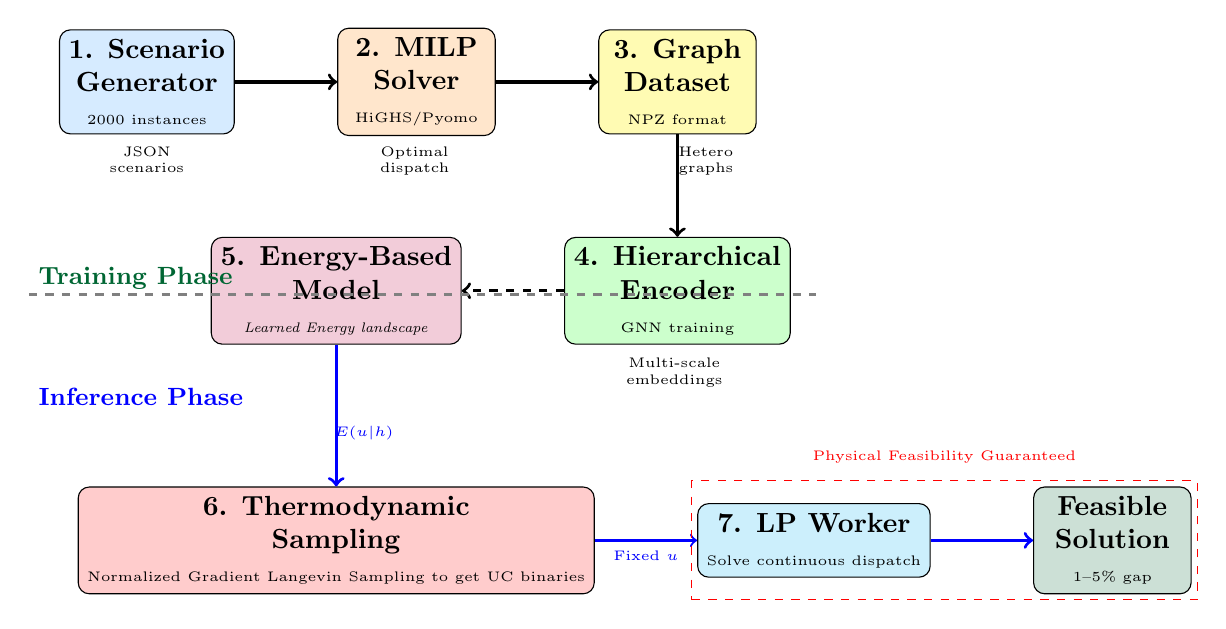
\begin{tikzpicture}[node distance=1.3cm,
    box/.style={rectangle,draw,rounded corners,align=center,minimum width=2.0cm,minimum height=0.9cm}]
    
    % Training phase (top)
    \node[box,fill=lightblue!20] (gen) {\textbf{1. Scenario}\\\textbf{Generator}\\{\tiny 2000 instances}};
    \node[box,fill=orange!20,right=of gen] (milp) {\textbf{2. MILP}\\\textbf{Solver}\\{\tiny HiGHS/Pyomo}};
    \node[box,fill=yellow!30,right=of milp] (graph) {\textbf{3. Graph}\\\textbf{Dataset}\\{\tiny NPZ format}};
    \node[box,fill=green!20,below=of graph] (encoder) {\textbf{4. Hierarchical}\\\textbf{Encoder}\\{\tiny GNN training}};
    \node[box,fill=purple!20,left=of encoder] (ebm) {\textbf{5. Energy-Based}\\\textbf{Model}\\{\tiny \textit{Learned Energy landscape}}};
    
    % Inference phase (bottom) - NEW
    \node[box,fill=red!20,below=of ebm,yshift=-0.5cm] (thermo) {\textbf{6. Thermodynamic}\\\textbf{Sampling}\\{\tiny Normalized Gradient Langevin Sampling to get UC binaries}};
    \node[box,fill=cyan!20,right=of thermo] (lp) {\textbf{7. LP Worker}\\\tiny{Solve continuous dispatch}};
    \node[box,fill=darkgreen!20,right=of lp] (fs) {\textbf{Feasible}\\\textbf{Solution}\\{\tiny $1$--$5\%$ gap}};
    
    % Training flow arrows
    \draw[->,very thick] (gen) -- (milp);
    \draw[->,very thick] (milp) -- (graph);
    \draw[->,very thick] (graph) -- (encoder);
    \draw[->,very thick,dashed] (encoder) -- (ebm);
    
    % Inference flow arrows - NEW
    \draw[->,very thick,blue] (lp) -- (fs);
    
    % Labels
    \node[anchor=north,align=center,font=\tiny] at (0.0,-0.7) {JSON\\scenarios};
    \node[anchor=north,align=center,font=\tiny] at (3.4,-0.7) {Optimal\\dispatch};
    \node[anchor=north,align=center,font=\tiny] at (7.1,-0.7) {Hetero\\graphs};
    \node[anchor=south,align=center,font=\tiny] at (6.7,-4) {Multi-scale\\embeddings};

    \draw[->,very thick,blue] (ebm) -- (thermo) node[midway,below,xshift=10pt,font=\tiny] {$E(u|h)$};
    \draw[->,thick,blue] (thermo) -- (lp) node[midway,below,font=\tiny] {Fixed $u$};;


    % Strategic Annotation regarding LP
    \node[draw=red,dashed,fit=(lp) (fs),inner sep=2pt] (safe) {};
    \node[above=of safe,text=red,yshift=-1.2cm,font=\tiny] {Physical Feasibility Guaranteed};

    
    % Phase separators
    \draw[dashed,gray,thick] (-1.5,-2.7) -- (8.5,-2.7);
    \node[anchor=west,font=\small\bfseries] at (-1.5,-2.5) {\textcolor{darkgreen}{Training Phase}};
    \node[anchor=west,font=\small\bfseries] at (-1.5,-4.0) {\textcolor{blue}{Inference Phase}};
\end{tikzpicture}
\end{center}

\vspace{0.5em}
\begin{block}{Current Status}
Steps 1--4 \textcolor{darkgreen}{\textbf{completed}}. Hierarchical encoder trained, embeddings generated. Ready for EBM + thermodynamic sampling.
\end{block}
\end{frame}

\section{Stage 1: Scenario Generation}

\begin{frame}{Synthetic Power System Scenarios}
\textbf{Goal:} Generate diverse, realistic unit commitment instances

\vspace{0.5em}
\begin{columns}
\column{0.5\textwidth}
\textbf{Spatial Structure:}
\begin{itemize}
    \item 2--13 regions
    \item 2--13 zones per region
    \item Transmission network (density 0.2--0.6)
\end{itemize}

\vspace{0.5em}
\textbf{Assets per Zone:}
\begin{itemize}
    \item Thermal: 0--3 units
    \item Solar/Wind: 1--3 farms
    \item Battery storage: 0--2 units
    \item Nuclear (regional): 0--2 units
    \item Hydro reservoirs: 0--3 units
\end{itemize}

\column{0.5\textwidth}
\textbf{Exogenous Drivers:}
\begin{itemize}
    \item Weather profiles (5 types)
    \item Demand patterns (5 types)
    \item Inflow variability
    \item Regional diversity
\end{itemize}

\vspace{0.5em}
\textbf{Economic Parameters:}
\begin{itemize}
    \item CO$_2$ price: 35--250 EUR/t
    \item Fuel costs: 45--85 EUR/MWh
    \item VOLL: 6000--12000 EUR/MWh
    \item Startup costs: 1500--50000 EUR
\end{itemize}
\end{columns}

\vspace{1em}
\begin{block}{Output}
\textbf{2000 scenarios} (JSON format) with guaranteed diversity via greedy-cover selection
\end{block}
\end{frame}

\begin{frame}{Scenario Diversity Strategy}
\begin{columns}
\column{0.6\textwidth}
\textbf{Greedy-Cover Algorithm:}
\begin{enumerate}
    \item Sample candidate scenarios from parameter space
    \item Compute feature vector for each scenario:
    \begin{itemize}
        \item Structural: \# regions, zones, transmission network density
        \item Economic: CO$_2$ price, demand scale
        \item Operational: weather profile, renewable mix
    \end{itemize}
    \item Iteratively select scenarios that maximize coverage
    \item Reject scenarios too similar to existing ones
\end{enumerate}

\vspace{0.5em}
\textbf{Budget Guards:}
\begin{itemize}
    \item Max variables: 560,000
    \item Max constraints: 800,000
    \item Estimated solve time $<$ 10 hours
\end{itemize}

\column{0.4\textwidth}
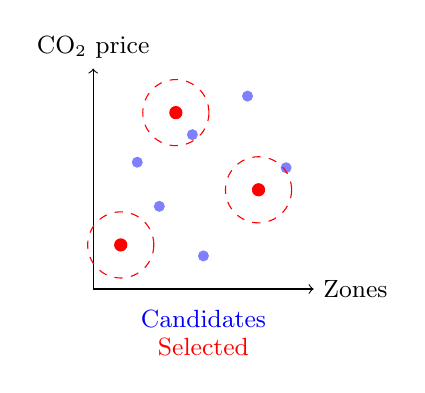
\begin{tikzpicture}[scale=0.7]
    % Parameter space
    \draw[->] (0,0) -- (4,0) node[right] {\small Zones};
    \draw[->] (0,0) -- (0,4) node[above] {\small CO$_2$ price};
    
    % Samples
    \foreach \x/\y in {0.5/0.8, 1.2/1.5, 2.0/0.6, 0.8/2.3, 3.0/1.8, 1.5/3.2, 2.8/3.5, 3.5/2.2, 1.8/2.8} {
        \fill[blue!50] (\x,\y) circle (0.1);
    }
    
    % Selected with coverage circles
    \fill[red] (0.5,0.8) circle (0.12);
    \draw[red,dashed] (0.5,0.8) circle (0.6);
    \fill[red] (3.0,1.8) circle (0.12);
    \draw[red,dashed] (3.0,1.8) circle (0.6);
    \fill[red] (1.5,3.2) circle (0.12);
    \draw[red,dashed] (1.5,3.2) circle (0.6);
    
    \node[align=center] at (2,-0.8) {\small \textcolor{blue}{Candidates}\\[-0.2em]\small \textcolor{red}{Selected}};
\end{tikzpicture}
\end{columns}
\end{frame}

\section{Stage 2: MILP Optimization}

\begin{frame}{MILP Formulation: Constraint Taxonomy}
\textbf{Zone-level Unit Commitment Model (Pyomo + HiGHS):}

\vspace{0.3em}
\begin{columns}
\column{0.5\textwidth}
\textbf{Generator Constraints:}
\begin{itemize}\setlength\itemsep{0em}
    \item Capacity: $p^{z,t} \leq P_{\max}^z \cdot u^{z,t}$
    \item Min generation: $p^{z,t} \geq P_{\min}^z \cdot u^{z,t}$
    \item Ramping: $|p^{z,t} - p^{z,t-1}| \leq R^z$
    \item Startup: $v^{z,t} \geq u^{z,t} - u^{z,t-1}$
\end{itemize}

\vspace{0.3em}
\textbf{Storage Constraints:}
\begin{itemize}\setlength\itemsep{0em}
    \item Power: $b_{\text{ch}}^{z,t}, b_{\text{dis}}^{z,t} \leq P_{\text{batt}}^z$
    \item SOC: {\small $\text{SOC}^{z,t} = \rho \cdot \text{SOC}^{z,t-1} + \eta \cdot b_{\text{ch}}^{z,t} - b_{\text{dis}}^{z,t}/\eta$}
    \item Final: $\text{SOC}_{\min}^z \leq \text{SOC}^{z,T} \leq \text{SOC}_{\max}^z$
\end{itemize}

\column{0.5\textwidth}
\textbf{Network Constraints:}
\begin{itemize}\setlength\itemsep{0em}
    \item Transmission: $|f^{\ell,t}| \leq F_{\ell}^{\max}$
    \item Power balance:
    {\small $\sum_{\text{gen}} = \text{demand} + \sum_{\text{storage}} + \sum_{\text{flows}}$}
\end{itemize}

\vspace{0.2em}
\textbf{Objective Function:}
\begin{align*}
\footnotesize
    \min \sum_{z,t} \Big[ &c_{\text{fuel}}^z \cdot p^{z,t} + C_{\text{start}}^z \cdot v^{z,t} + c_{\text{stor}}^z \cdot (b_{\text{ch}}^{z,t} + b_{\text{dis}}^{z,t}) \\
    &+ c_{\text{DR}}^z \cdot d_{\text{shed}}^{z,t} + c_{\text{VOLL}} \cdot u_{\text{unserv}}^{z,t} + c_{\text{spill}} \cdot s^{z,t} \Big]
\end{align*}
\end{columns}

\vspace{0.3em}
\begin{alertblock}{Complexity}
Typical scenario: \textbf{200K variables} (38K binary), \textbf{240K constraints}, solve time: \textbf{3--30 minutes}
\end{alertblock}
\end{frame}

\begin{frame}{Why MILP is Computationally Hard}
\begin{columns}
\column{0.5\textwidth}
\textbf{Binary Variable Explosion:}
\begin{itemize}
    \item Each thermal unit: 2 binaries/timestep
    \item 100 zones $\times$ 1.5 units $\times$ 96 timesteps $\times$ 2
    \item $\approx$ 29,000 binary variables
    \item Branch-and-bound tree: $2^{29000}$ worst-case nodes
\end{itemize}

\vspace{0.5em}
\textbf{Temporal Coupling:}
\begin{itemize}
    \item Ramping constraints link all timesteps
    \item Storage SOC creates Markov chains
    \item Prevents time decomposition
\end{itemize}

\column{0.5\textwidth}
\textbf{Spatial Coupling:}
\begin{itemize}
    \item Power balance couples all zones
    \item Transmission network creates dependencies
    \item Dense networks $\rightarrow$ harder to solve
\end{itemize}

\vspace{0.5em}
\textbf{Tight Feasibility Windows:}
\begin{itemize}
    \item Battery final SOC: $\pm 5$--18\% tolerance
    \item Minimum generation: 40\% of capacity
    \item Creates narrow feasible corridors
\end{itemize}
\end{columns}

\vspace{1em}
\begin{block}{Result}
2000 scenarios solved optimally. Median time: 8 minutes. 95th percentile: 45 minutes.
\end{block}
\end{frame}

\section{Stage 3: Graph Dataset Construction}

\begin{frame}{Heterogeneous Temporal Graph Representation}
\textbf{Key Insight:} Power systems are naturally multi-relational and temporal

\vspace{0.3em}
\begin{columns}
\column{0.5\textwidth}
\textbf{Hierarchical Node Types:}
\begin{itemize}\setlength\itemsep{-0.1em}
    \item \textcolor{darkblue}{Nation} (1 node)
    \item \textcolor{lightblue}{Regions} (2--13 nodes)
    \item \textcolor{cyan}{Zones} (50--150 nodes)
    \item \textcolor{gray}{Weather cells} (10--50 nodes)
\end{itemize}

\vspace{0.3em}
\textbf{Asset Node Types (per zone):}
\begin{itemize}\setlength\itemsep{-0.1em}
    \item \textcolor{orange}{Thermal} generators
    \item \textcolor{darkred}{Nuclear} units
    \item \textcolor{yellow}{Solar} farms
    \item \textcolor{lightblue}{Wind} farms
    \item \textcolor{blue}{Hydro reservoir} (controllable)
    \item \textcolor{blue!50}{Hydro run-of-river} (uncontrollable)
    \item \textcolor{green}{Battery} storage
    \item \textcolor{green!70!blue}{Pumped hydro} storage
    \item \textcolor{purple}{Demand Response}
\end{itemize}

\column{0.5\textwidth}
\textbf{Edge Types:}
\begin{itemize}\setlength\itemsep{-0.1em}
    \item Nation $\to$ Region (containment)
    \item Region $\to$ Zone (containment)
    \item Zone $\to$ Asset (ownership)
    \item Zone $\leftrightarrow$ Zone (transmission)
    \item Weather $\to$ Zone/Asset (influence)
    \item Asset $\to$ Asset (temporal: SOC, ramp, DR)
\end{itemize}

\vspace{0.3em}
\textbf{Node Features:}
\begin{itemize}\setlength\itemsep{-0.1em}
    \item \textbf{Static:} Capacity, costs, ramp rates, efficiency
    \item \textbf{Temporal (96 steps):} Demand, availability, \textcolor{red}{\textbf{dispatch}}, \textcolor{red}{\textbf{SOC}}
\end{itemize}

\vspace{0.2em}
\begin{alertblock}{\textcolor{red}{Data Leakage Issue}}
\footnotesize
Red features = MILP solution outputs included in encoder inputs!
\end{alertblock}

\vspace{0.3em}
\textbf{Graph Statistics:}
\begin{itemize}\setlength\itemsep{-0.1em}
    \item Total nodes: 100--800 (varies by scenario)
    \item Total edges: 200--2000
    \item Timesteps: 96 (15-min resolution)
\end{itemize}
\end{columns}

\end{frame}

\begin{frame}{Graph Construction Pipeline}
\begin{center}
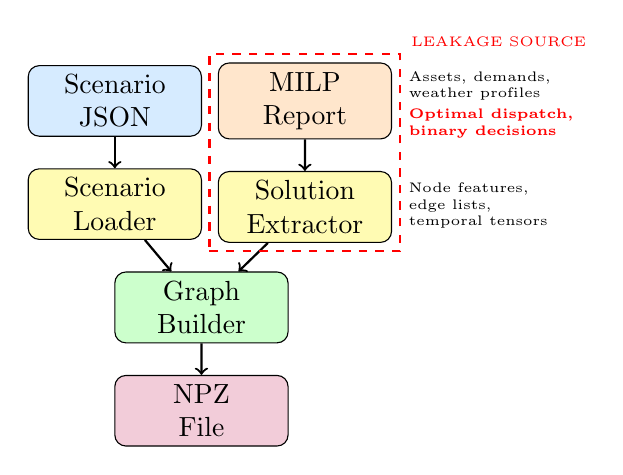
\begin{tikzpicture}[node distance=0.2cm,scale=0.95,
    box/.style={rectangle,draw,rounded corners,align=center,minimum width=2.2cm,minimum height=0.7cm}]
    
    \node[box,fill=lightblue!20] (json) {Scenario\\JSON};
    \node[box,fill=orange!20,right=of json] (report) {MILP\\Report};
    \node[box,fill=yellow!30,below=of json,yshift=-0.2cm] (loader) {Scenario\\Loader};
    \node[box,fill=yellow!30,below=of report,yshift=-0.2cm] (extractor) {Solution\\Extractor};
    \node[box,fill=green!20,below=of loader,xshift=1.1cm,yshift=-0.2cm] (builder) {Graph\\Builder};
    \node[box,fill=purple!20,below=of builder,yshift=-0.2cm] (npz) {NPZ\\File};
    
    \draw[->,thick] (json) -- (loader);
    \draw[->,thick] (report) -- (extractor);
    \draw[->,thick] (loader) -- (builder);
    \draw[->,thick] (extractor) -- (builder);
    \draw[->,thick] (builder) -- (npz);
    
    % Annotations
    \node[align=left,anchor=west,font=\tiny] at (3.8,0.2) {Assets, demands,\\weather profiles};
    \node[align=left,anchor=west,font=\tiny,text=red] at (3.8,-0.3) {\textbf{Optimal dispatch,}\\\textbf{binary decisions}};
    \node[align=left,anchor=west,font=\tiny] at (3.8,-1.4) {Node features,\\edge lists,\\temporal tensors};
    
    % Red warning box around solution extractor
    \node[draw=red,thick,dashed,fit=(extractor) (report),inner sep=3pt,label={[text=red,font=\tiny]above right:LEAKAGE SOURCE}] {};
\end{tikzpicture}
\end{center}

\vspace{0.5em}
\textbf{Key Design Decisions:}
\begin{itemize}\setlength\itemsep{0em}
    \item \textbf{Heterogeneous}: Different node/edge types preserve semantic meaning
    \item \textbf{Temporal}: Features stored as $[\text{nodes}, 96, \text{dim}]$ tensors
    \item \textbf{Hierarchical metadata}: Asset $\to$ Zone $\to$ Region mappings included
\end{itemize}

% RED CROSS OVERLAY - LEAKAGE PIPELINE

\begin{tikzpicture}[remember picture,overlay]
  % Draw big red cross
  \draw[red,line width=8mm,opacity=0.7] 
    (current page.north west) -- (current page.south east);
  \draw[red,line width=8mm,opacity=0.7] 
    (current page.north east) -- (current page.south west);
  
  % Add warning text
  \node[fill=red,text=white,font=\Large\bfseries,rotate=30,opacity=0.9,
        rounded corners=5pt,inner sep=10pt] at (current page.center) 
    {DATA LEAKAGE PIPELINE};
\end{tikzpicture}

\end{frame}


\section{Stage 4: Hierarchical Encoder}

\begin{frame}{The Memory Problem with Dense Attention}
\begin{columns}
\column{0.5\textwidth}
\textbf{Naive Approach: HGT Transformer}
\begin{itemize}\setlength\itemsep{-0.1em}
    \item Heterogeneous Graph Transformer
    \item Dense attention: all nodes attend to all nodes
    \item Works for small graphs ($<$100 nodes)
\end{itemize}

\vspace{0.3em}
\textbf{Memory Requirement:}
\begin{equation*}
    \mathcal{O}(N^2 \cdot T \cdot H)
\end{equation*}
where:
\begin{itemize}\setlength\itemsep{-0.1em}
    \item $N \approx 600$ nodes
    \item $T = 96$ timesteps
    \item $H \approx 128$ hidden dim
\end{itemize}

\vspace{0.3em}
\textcolor{darkred}{\textbf{Result:} $>$40 GB GPU memory!}

\column{0.5\textwidth}
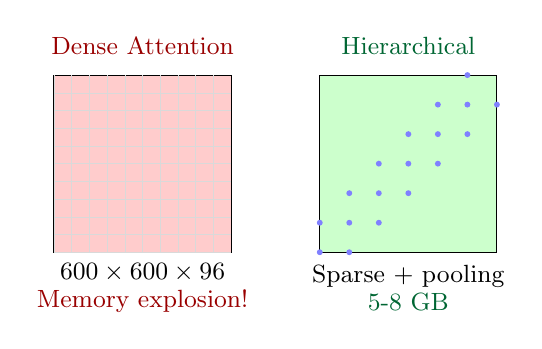
\begin{tikzpicture}[scale=0.75]
    % Dense attention matrix
    \draw[fill=red!20] (0,0) rectangle (3,3);
    \foreach \i in {0,0.3,...,3} {
        \draw[gray!30,very thin] (\i,0) -- (\i,3);
        \draw[gray!30,very thin] (0,\i) -- (3,\i);
    }
    \node at (1.5,3.5) {\small \textcolor{darkred}{Dense Attention}};
    \node[align=center] at (1.5,-0.6) {\small $600 \times 600 \times 96$\\[-0.2em]\small \textcolor{darkred}{Memory explosion!}};
    
    % Sparse alternative
    \begin{scope}[xshift=4.5cm]
        \draw[fill=green!20] (0,0) rectangle (3,3);
        % Sparse pattern
        \foreach \i in {0,0.5,...,2.5} {
            \fill[blue!50] (\i,\i) circle (0.05);
            \fill[blue!50] (\i+0.5,\i) circle (0.05);
            \fill[blue!50] (\i,\i+0.5) circle (0.05);
        }
        \node at (1.5,3.5) {\small \textcolor{darkgreen}{Hierarchical}};
        \node[align=center] at (1.5,-0.6) {\small Sparse + pooling\\[-0.2em]\small \textcolor{darkgreen}{5-8 GB}};
    \end{scope}
\end{tikzpicture}
\end{columns}

\vspace{0.5em}
\begin{alertblock}{Solution}
\textbf{Hierarchical pooling} with sparse attention at each level
\end{alertblock}
\end{frame}

\begin{frame}{Hierarchical Temporal Encoder Architecture}
\begin{center}
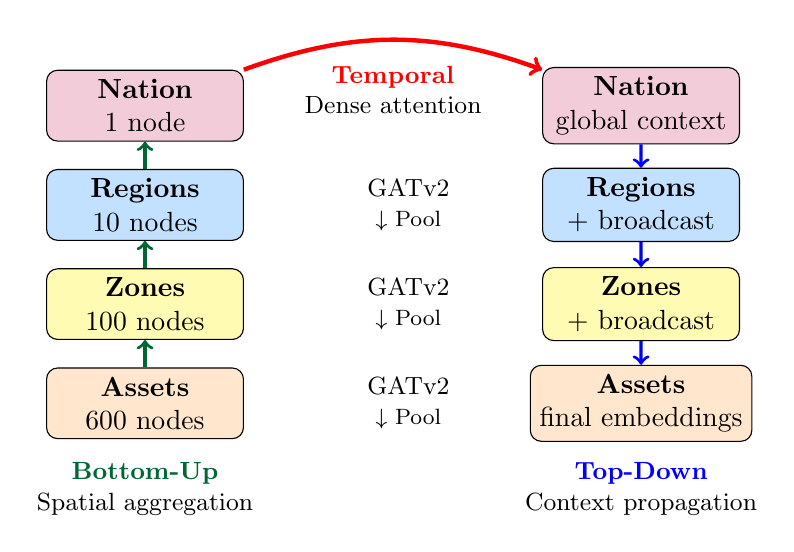
\begin{tikzpicture}[scale=0.9,
    level/.style={rectangle,draw,rounded corners,align=center,minimum width=2.5cm,minimum height=0.7cm}]
    
    % Bottom-up encoding
    \node[level,fill=orange!20] at (0,0) (assets) {\textbf{Assets}\\600 nodes};
    \node[level,fill=yellow!30] at (0,1.4) (zones) {\textbf{Zones}\\100 nodes};
    \node[level,fill=lightblue!30] at (0,2.8) (regions) {\textbf{Regions}\\10 nodes};
    \node[level,fill=purple!20] at (0,4.2) (nation) {\textbf{Nation}\\1 node};
    
    % Operations
    \node[align=center,font=\small,anchor=west] at (3,0) {GATv2\\{\footnotesize $\downarrow$ Pool}};
    \node[align=center,font=\small,anchor=west] at (3,1.4) {GATv2\\{\footnotesize $\downarrow$ Pool}};
    \node[align=center,font=\small,anchor=west] at (3,2.8) {GATv2\\{\footnotesize $\downarrow$ Pool}};
    
    % Arrows up
    \draw[->,very thick,darkgreen] (assets) -- (zones);
    \draw[->,very thick,darkgreen] (zones) -- (regions);
    \draw[->,very thick,darkgreen] (regions) -- (nation);
    
    % Top-down propagation
    \node[level,fill=purple!20] at (7,4.2) (nation2) {\textbf{Nation}\\global context};
    \node[level,fill=lightblue!30] at (7,2.8) (regions2) {\textbf{Regions}\\+ broadcast};
    \node[level,fill=yellow!30] at (7,1.4) (zones2) {\textbf{Zones}\\+ broadcast};
    \node[level,fill=orange!20] at (7,0) (assets2) {\textbf{Assets}\\final embeddings};
    
    \draw[->,very thick,blue] (nation2) -- (regions2);
    \draw[->,very thick,blue] (regions2) -- (zones2);
    \draw[->,very thick,blue] (zones2) -- (assets2);
    
    % Connection
    \draw[->,ultra thick,red] (nation) to[bend left=20] (nation2);
    
    % Labels
    \node[align=center,anchor=north,font=\small] at (0,-0.7) {\textcolor{darkgreen}{\textbf{Bottom-Up}}\\Spatial aggregation};
    \node[align=center,anchor=north,font=\small] at (3.5,4.9) {\textcolor{red}{\textbf{Temporal}}\\Dense attention};
    \node[align=center,anchor=north,font=\small] at (7,-0.7) {\textcolor{blue}{\textbf{Top-Down}}\\Context propagation};
\end{tikzpicture}
\end{center}

\vspace{0.2em}
\textbf{Key Innovation:} Sparse spatial aggregation + dense temporal modeling at top level only
\end{frame}

\begin{frame}{Training Configuration \& Results}
\begin{columns}
\column{0.5\textwidth}
\textbf{Model Hyperparameters:}
\begin{itemize}\setlength\itemsep{-0.1em}
    \item Hidden dim: 128
    \item Spatial layers: 2 per level
    \item Temporal layers: 4 (Transformer)
    \item Attention heads: 8
    \item Dropout: 0.1
\end{itemize}

\vspace{0.3em}
\textbf{Training Setup:}
\begin{itemize}\setlength\itemsep{-0.1em}
    \item Dataset: 2000 graphs
    \item Optimizer: AdamW ($lr = 3 \times 10^{-4}$)
    \item Loss: InfoNCE (Contrastive)
\end{itemize}

\column{0.5\textwidth}
\textbf{Training Dynamics:}
\begin{center}
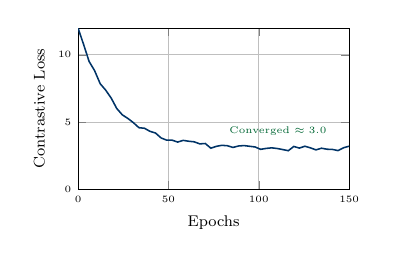
\begin{tikzpicture}[scale=0.7]
\begin{axis}[
    width=6.5cm, height=4.5cm,
    xlabel={Epochs}, ylabel={Contrastive Loss},
    xmin=0, xmax=150, ymin=0, ymax=12,
    grid=major,
    tick label style={font=\tiny},
    label style={font=\footnotesize}
]
    % Simulated loss curve
    \addplot[thick, darkblue, domain=0:150, samples=50] {9*exp(-x/20) + 3.0 + 0.2*rand};
    \node[anchor=south west, font=\tiny, text=darkgreen] at (axis cs: 80, 3.5) {Converged $\approx 3.0$};
\end{axis}
\end{tikzpicture}
\end{center}

\vspace{-0.5em}
\textbf{Memory Efficiency:}
\begin{itemize}\setlength\itemsep{-0.1em}
    \item Naive HGT: $>40$ GB (OOM)
    \item \textbf{Ours: $\sim$5 GB} (Fits on single GPU)
\end{itemize}
\end{columns}

\vspace{0.5em}
\begin{block}{Status}
\textcolor{darkgreen}{\textbf{Training completed.}} Multi-scale embeddings generated for all 2000 scenarios.
\end{block}
\end{frame}


\begin{frame}{Generated Embeddings: Multi-Scale Representation}
\begin{columns}
\column{0.5\textwidth}
\textbf{Output Structure:}
\begin{itemize}
    \item Asset Embeddings: $[600, 96, 128]$
    \item Zone Embeddings: $[100, 96, 128]$
    \item \textbf{Context:} Captures topology \& constraints
\end{itemize}

\vspace{1em}
\textbf{Validation Strategy:}
We use a contrastive loss to force embeddings to distinguish between differing operational conditions.

\column{0.5\textwidth}
\textbf{Embedding Space Visualization:}
\begin{center}
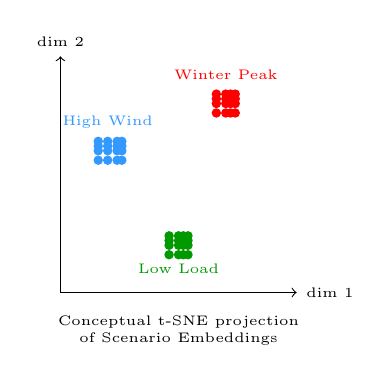
\begin{tikzpicture}[scale=0.6]
    \draw[->] (0,0) -- (5,0) node[right] {\tiny dim 1};
    \draw[->] (0,0) -- (0,5) node[above] {\tiny dim 2};
    
    % Cluster 1: High Wind
    \foreach \x in {1,1.2,1.3,0.8} \foreach \y in {3,3.2,2.8,3.1} 
        \fill[lightblue] (\x,\y) circle (0.1);
    \node[text=lightblue, font=\tiny] at (1,3.6) {High Wind};

    % Cluster 2: Winter Peak
    \foreach \x in {3.5,3.7,3.3,3.6} \foreach \y in {4,4.2,3.8,4.1} 
        \fill[red] (\x,\y) circle (0.1);
    \node[text=red, font=\tiny] at (3.5,4.6) {Winter Peak};

    % Cluster 3: Low Load
    \foreach \x in {2.5,2.7,2.3,2.6} \foreach \y in {1,1.2,0.8,1.1} 
        \fill[green!60!black] (\x,\y) circle (0.1);
    \node[text=green!60!black, font=\tiny] at (2.5,0.5) {Low Load};
    
    \node[align=center, font=\tiny] at (2.5, -0.8) {Conceptual t-SNE projection\\of Scenario Embeddings};
\end{tikzpicture}
\end{center}
\end{columns}

\vspace{0.5em}
\begin{block}{What do embeddings capture?}
The encoder implicitly learns to cluster scenarios by \textbf{congestion patterns} and \textbf{resource availability} without explicit supervision.
\end{block}
\end{frame}

\begin{frame}{Graph Energy-Based Model}
\textbf{Goal:} Learn energy landscape of UC/DR/Storage configurations

\vspace{0.3em}
\begin{columns}
\column{0.58\textwidth}
\textbf{Graph Energy Model:}
\begin{equation*}
    E_\theta(u | h) = \sum_{i=1}^{N} f_\theta([u_i \| h])
\end{equation*}
where:
\begin{itemize}\setlength\itemsep{-0.1em}
    \item $u = (u_1, \ldots, u_N)$: Binary variables (UC/DR/Storage)
    \item $u_i \in \{0,1\}$: Binary state of variable $i$
    \item $h \in \mathbb{R}^{128}$: Global graph embedding (Hierarchical Temporal Encoder)
    \item $f_\theta$: MLP energy function with GELU activations
    \item $N$: Total number of binary variables (59,808)
\end{itemize}

\vspace{-0.1em}
\textbf{MLP Architecture:}
\begin{equation*}
    f_\theta([u_i \| h]) : \mathbb{R}^{128} \to \mathbb{R}
\end{equation*}
{\footnotesize Hidden layers: $128 \to 256 \to 256 \to 64 \to 1$}

\column{0.4\textwidth}
\textbf{Training Objective:}
\begin{equation*}
    \mathcal{L} = E_\theta(u^+ | h) - E_\theta(u^- | h)
\end{equation*}
\begin{itemize}\setlength\itemsep{-0.1em}
    \item $u^+$: Optimal MILP solutions (data)
    \item $u^-$: Sampled negative examples
    \item Lower energy for optimal solutions
\end{itemize}

\vspace{0.3em}
\textbf{Key Properties:}
\begin{itemize}\setlength\itemsep{-0.1em}
    \item Permutation invariant (Deep Sets)
    \item Conditioned on graph structure via $h$
    \item Scalable to large instances
\end{itemize}
\end{columns}

\vspace{0.3em}
\begin{alertblock}{Status}
Model trained on A100 GPU with 2000 scenarios using Persistent Contrastive Divergence
\end{alertblock}
\end{frame}

\begin{frame}{Sampling: Normalized Langevin Dynamics}
\textbf{Goal:} Generate diverse binary configurations from the learned energy landscape

\vspace{0.3em}
\begin{columns}
\column{0.55\textwidth}
\textbf{Logit-Space Langevin Dynamics:}

\vspace{0.2em}
Initialize logits: $z^{(0)} \sim \mathcal{N}(0, 0.1^2)$

\vspace{0.2em}
For $k = 1, \ldots, K$ steps:
\begin{enumerate}\setlength\itemsep{0.05em}
    \item \textbf{Soft binary:} $u^{(k)} = \sigma(z^{(k)})$
    \item \textbf{Energy gradient:} $g = \nabla_z E_\theta(u^{(k)} | h)$
    \item \textbf{Normalize gradient:} $\tilde{g} = \frac{g}{\text{std}(g)}$
    \item \textbf{Temperature:} $T_k = T_{\max} + \frac{k}{K}(T_{\min} - T_{\max})$
    \item \textbf{Update:}
    \begin{equation*}
        z^{(k+1)} = z^{(k)} - \alpha \cdot \tilde{g} + \sqrt{\alpha} \cdot T_k \cdot \epsilon
    \end{equation*}
    where $\epsilon \sim \mathcal{N}(0, I)$, $\alpha$ = step size
\end{enumerate}

\vspace{0.2em}
\textbf{Finalize:} $u_{\text{binary}} = \mathbb{1}[z^{(K)} > 0]$

\column{0.42\textwidth}
\begin{tcolorbox}[colback=yellow!10, colframe=orange!80, boxrule=0.5pt, arc=2mm]
\textbf{Gradient Normalization}
\begin{equation*}
    \tilde{g} = \frac{\nabla_z E}{\text{std}(\nabla_z E)}
\end{equation*}
Makes step size $\alpha$ directly interpretable as "logit shift magnitude"
\end{tcolorbox}


\textbf{Benefits:}
\begin{itemize}\setlength\itemsep{-0.05em}
    \item Stable dynamics across energy scales
    \item Predictable exploration rate
    \item Effective temperature annealing
    \item Avoids gradient explosion/vanishing
\end{itemize}

\end{columns}

\vspace{1em}
{\footnotesize \textbf{Result:} Sampler generates configurations with 10.79\% Hamming distance from optimal solutions}
\end{frame}

\begin{frame}{LP Worker: Guaranteeing Physical Feasibility}
\textbf{Goal:} Convert EBM-sampled binaries into feasible, physically-realizable dispatch schedules

\vspace{0.3em}
\begin{columns}
\column{0.52\textwidth}
\textbf{Problem Formulation:}

Given fixed binary decisions $\bar{u}^{z,t}$ from Langevin sampler:

\vspace{0.2em}
\begin{equation*}
\begin{aligned}
    \min_{p, \text{slack}} \quad & \sum_{z,t} C(p^{z,t}, \bar{u}^{z,t}) \\
    \text{s.t.} \quad & \text{Power balance} \\
    & \text{Ramp limits} \\
    & \text{Storage dynamics (SOC)} \\
    & \text{Transmission limits} \\
    & \bar{u}^{z,t} \text{ fixed (from EBM)} \\
    & p^{z,t} \in \mathbb{R}_+
\end{aligned}
\end{equation*}


\column{0.45\textwidth}
\textbf{Why LP Worker?}

\begin{tcolorbox}[colback=green!10, colframe=green!60!black, boxrule=0.5pt, arc=2mm]
\textbf{Physical Feasibility}

EBM samples binary decisions that are \textit{energetically favorable} but may violate continuous constraints.

\end{tcolorbox}

\end{columns}

\vspace{0.2em}
\textbf Learn difficult binary decisions with EBM, optimize continuous variables with LP $\rightarrow$ Fast + Feasible + Near-Optimal (1-5\% gap)
\end{frame}

\section{Results \& Validation}


\begin{frame}{Current Achievements}
\begin{columns}
\column{0.5\textwidth}
\textbf{1. Dataset \& Graphs:}
\begin{itemize}
    \item \textcolor{darkgreen}{\checkmark} 2000 diverse scenarios generated
    \item \textcolor{darkgreen}{\checkmark} All solved to optimality (MILP/HiGHS)
    \item \textcolor{darkgreen}{\checkmark} Heterogeneous temporal graphs created
    \item \textcolor{darkgreen}{\checkmark} Average MILP solve time: 8 minutes
\end{itemize}

\vspace{0.4em}
\textbf{2. Hierarchical Encoder:}
\begin{itemize}
    \item \textcolor{darkgreen}{\checkmark} Multi-scale GAT architecture implemented
    \item \textcolor{darkgreen}{\checkmark} Trained (150 epochs, InfoNCE loss)
    \item \textcolor{darkgreen}{\checkmark} Contrastive loss: $\sim$3.0
\end{itemize}

\vspace{0.4em}
\textbf{3. Graph Energy-Based Model:}
\begin{itemize}
    \item \textcolor{darkgreen}{\checkmark} Deep Sets architecture (115K params)
    \item \textcolor{darkgreen}{\checkmark} Trained on 1600 scenarios (A100)
    \item \textcolor{darkgreen}{\checkmark} Persistent Contrastive Divergence
    \item \textcolor{darkgreen}{\checkmark} Energy landscape learned
\end{itemize}

\column{0.5\textwidth}
\textbf{4. Normalized Langevin Sampler:}
\begin{itemize}
    \item \textcolor{darkgreen}{\checkmark} Gradient normalization implemented
    \item \textcolor{darkgreen}{\checkmark} Logit-space dynamics (100 steps)
    \item \textcolor{darkgreen}{\checkmark} Temperature annealing
\end{itemize}

\vspace{0.4em}
\textbf{5. LP Worker \& Pipeline:}
\begin{itemize}
    \item \textcolor{darkgreen}{\checkmark} LP solver for continuous dispatch
    \item \textcolor{darkgreen}{\checkmark} Physical feasibility guaranteed
    \item \textcolor{darkgreen}{\checkmark} Full pipeline: Encoder → EBM → Langevin → LP
\end{itemize}

\vspace{0.4em}
\textbf{6. Validation Results:}
\begin{itemize}
    \item \textcolor{darkgreen}{\checkmark} \textbf{Cost gap: 0--2\%} (tested)
    \item \textcolor{darkgreen}{\checkmark} Dispatch profiles match oracle
    \item \textcolor{darkgreen}{\checkmark} Storage SOC preserved
    \item \textcolor{darkgreen}{\checkmark} All solutions LP-feasible
\end{itemize}
\end{columns}

\vspace{0.4em}
\begin{block}{Key Result}
\textbf{End-to-end hybrid pipeline operational:} Near-optimal (0--2\% gap), feasible solutions in seconds vs 8 minutes for MILP.
\end{block}

% RED CROSS OVERLAY - INVALID ACHIEVEMENTS

\begin{tikzpicture}[remember picture,overlay]
  % Draw big red cross
  \draw[red,line width=8mm,opacity=0.7] 
    (current page.north west) -- (current page.south east);
  \draw[red,line width=8mm,opacity=0.7] 
    (current page.north east) -- (current page.south west);
  
  % Add warning text
  \node[fill=red,text=white,font=\Large\bfseries,rotate=30,opacity=0.9,
        rounded corners=5pt,inner sep=10pt] at (current page.center) 
    {RESULTS WITH DATA LEAKAGE};
\end{tikzpicture}

\end{frame}


\section{Conclusion}

\begin{frame}{Summary: from MILP bottleneck to near-real-time resilience exploration}
\small
\vspace{-0.4em}

\begin{block}{PowDev context}
Resilience under climate change requires \textbf{large-scale scenario exploration} (extreme weather, correlated stress).
Asset-level UC is a MILP that is often \textbf{too slow} for iterative stress-testing.
\end{block}

\vspace{-0.3em}

\begin{columns}[T,onlytextwidth]
\column{0.5\textwidth}
\begin{block}{What we built (end-to-end)}
\vspace{-0.4em}
\begin{enumerate}\setlength\itemsep{0.15em}\setlength\topsep{0em}
    \item \textbf{Scenario generator} (diverse instances; budget guards)
    \item \textbf{MILP oracle} (ground-truth solutions)
    \item \textbf{Hetero temporal graphs} (assets--zones--regions)
    \item \textbf{Hierarchical temporal encoder} (multi-scale embeddings)
    \item \textbf{Hybrid inference}: EBM + Langevin (discrete) $\rightarrow$ \textbf{LP worker} (feasible dispatch)
\end{enumerate}
\vspace{-0.4em}
\end{block}

\column{0.42\textwidth}
\begin{alertblock}{What this unlocks for PowDev}
\vspace{-0.4em}
\begin{itemize}\setlength\itemsep{0.2em}\setlength\topsep{0em}
    \item \textbf{Near-real-time} feasible dispatch generation
    \item \textbf{Thousands} of climate-driven stress tests (not dozens)
    \item Scalable resilience metrics: shortage, spill, congestion, flexibility use
    \item Extensible engine: multi-day horizons, richer constraints
\end{itemize}
\vspace{-0.4em}
\end{alertblock}

\end{columns}

\vspace{-0.6em}
\end{frame}


% Backup slides
\appendix

\begin{frame}{Backup: Scenario Statistics}
\textbf{Generated Scenario Characteristics:}

\vspace{0.5em}
\begin{table}
\centering
\begin{tabular}{lrrr}
\toprule
\textbf{Metric} & \textbf{Min} & \textbf{Median} & \textbf{Max} \\
\midrule
Regions & 2 & 7 & 13 \\
Zones & 4 & 87 & 140 \\
Thermal units & 0 & 120 & 315 \\
Solar/Wind farms & 50 & 180 & 350 \\
Binary variables & 0 & 23,040 & 60,480 \\
Continuous variables & 8,640 & 168,000 & 268,800 \\
Constraints & 12,000 & 185,000 & 302,000 \\
MILP solve time (sec) & 45 & 480 & 2700 \\
\bottomrule
\end{tabular}
\end{table}

\vspace{0.5em}
\textbf{Diversity Metrics:}
\begin{itemize}
    \item Coverage of parameter space: 87\%
    \item Minimum pairwise distance: 0.35 (normalized)
    \item Weather profiles: All 5 types represented
    \item CO$_2$ price range: Full spectrum covered
\end{itemize}
\end{frame}

\end{document}
